%!TEX encoding = IsoLatin

%% Document is article 
\documentclass[a4paper]{article}

%% ----------------------------------------------------- PACKAGES ----------------------------------------------------- %%
\usepackage{coolArticle}
\usepackage{optidef}

%% ---------------------------------------------------- DOCUMENT ---------------------------------------------------- %%
\begin{document}

\noindent \textsc{Gallos-Montbrun} Gr�goire\\
\textsc{Faury} Louis 
\vspace{15pt}

	\titlebox{0.6}{\Large Model Predictive Control}{\Large \textbf{\textcolor{blue}{Building Temperature Regulation}}}
	
	\section{Introduction}
	{
		\paragraph{} This project aims at controlling the temperature inside a 3 room building. The full state and output dynamics are given by : 
		\begin{equation}
			\begin{aligned}
				x^+ &= Ax + B_uu + B_dd\\
				y &= Cx
			\end{aligned}
		\end{equation}
		where : 
		\begin{equation}
		\left\{
			\begin{aligned}
				&x \in \mathbb{R}^{10} & &\text{ has no significant physical meaning} \\
				&u \in\mathbb{R}^3 & &\text{ is the electrical power dedicated to the heating of each room}\\
				&d \in\mathbb{R}^3 & &\text{ is the disturbance input (temperature, solar gain and internal gains)} \\
				&y\in\mathbb{R}^3 & & \text{ is the temperature in each room of the building}
			\end{aligned}\right.
		\end{equation}
		
		\paragraph{} The disturbance will be considered as an input, since we have its prediction over a period of 8 days. Figure (\ref{fig::temp_pred}) and (\ref{fig::gain_pred}) provides a plot of those predictive value. We can namely notice that we observe a \emph{\textcolor{red}{circadian periodicity}} (periodicity of 24h for the different signals). 
		
		\begin{figure}[h!]
			\begin{minipage}{0.45\linewidth}
				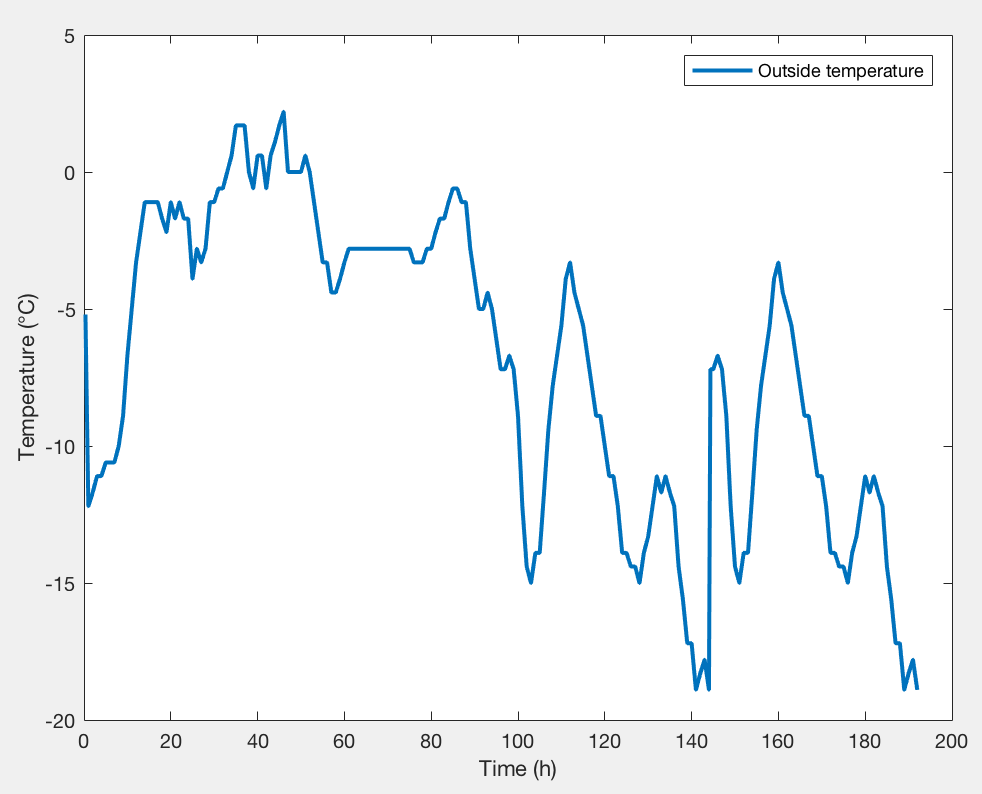
\includegraphics[width=\linewidth]{temp_pred}
				\caption{External temperature predictions}
				\label{fig::temp_pred}
			\end{minipage}
			\begin{minipage}{0.45\linewidth}
				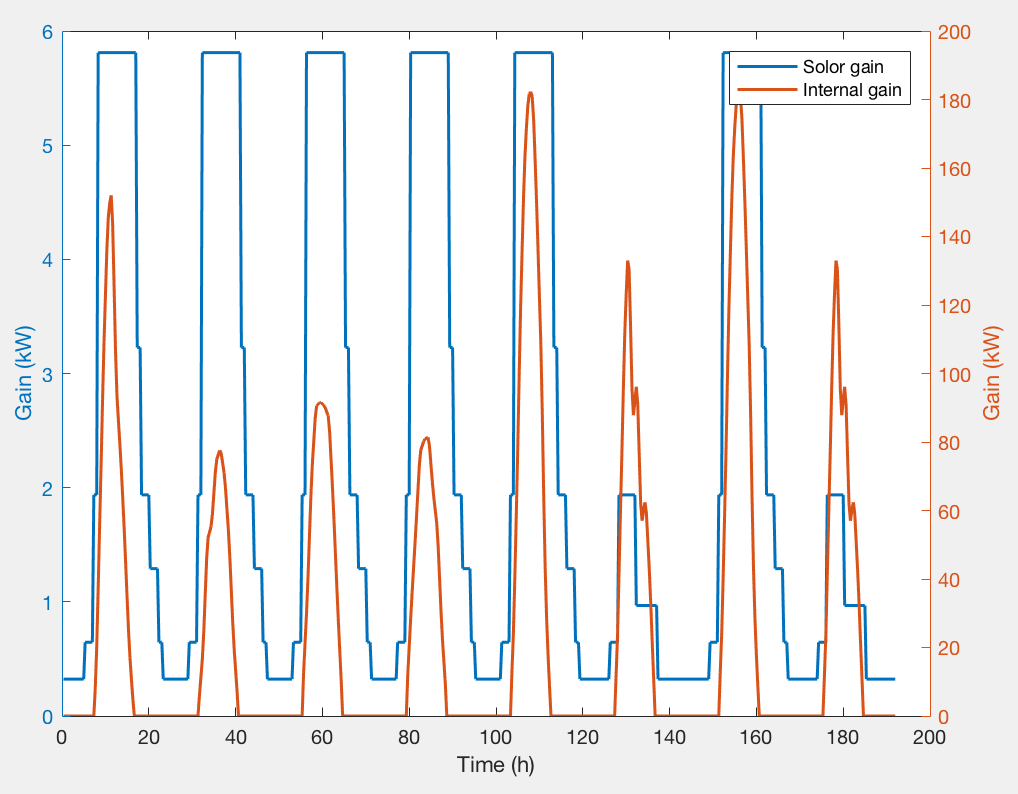
\includegraphics[width=\linewidth]{gains_pred}
				\caption{Solar and internal gain predictions}
				\label{fig::gain_pred}
			\end{minipage}
		\end{figure}
		
		\paragraph{} The following sections implements different versions of model predictive controllers, considering different objectives : target tracking, cost minimization, storage cost, .. 
	}
	
	\section{First MPC Controller}
	{
		\paragraph{} In this section, we are using YALMIP in order to design a MPC controller. This controller must regulate the output of the system around the reference output : 
		\begin{equation}
			y_r = \begin{pmatrix} 24 & 24 & 24 \end{pmatrix}
		\end{equation}
		by optimizing the cost function : 
		\begin{equation}
			J = \sum_{n=1}^N (y_n-y_r)^T R (y-y_n)
		\end{equation}
		under the following constraints : 
		\begin{equation}
			\begin{aligned}
				& y_n \geq 22, \quad & &n\in\{1,\hdots,N\} \\
				& y_n \leq 26, \quad & &n\in\{1,\hdots,N\} \\
				& u_n \leq 15, \quad & &n\in\{1,\hdots,N\} \\												& u_n \geq 0, \quad & &n\in\{1,\hdots,N\} \\
			\end{aligned}
		\end{equation}
		In the following, $R$ is chosen to be $\mathds{1}_3$ (hence we are penalizing equally any fluctuations around the target value, independently of the room). Given a cost function, multiplying $R$ by a scalar value won't have any effect on the optimal solution. 
		\newline We decided \emph{not to implement} a terminal cost nor terminal set constraints. This was mainly motivated by the fact that even with small horizons $N$, the system is \emph{experimentally} stable and recursively feasible. Hence, given the fact that the control invariant set could be computationally challenging to compute, and because its use would reduce the attraction zone in our state space, there was no real need to use terminal cost or terminal set. Moreover, the system is \emph{extremely reactive}, therefore we are able to reach, even with small horizons,  a cost that approximates the infinite horizon cost. 
		
		\paragraph{} Figures (\ref{fig::naivempc_N5_output}) and (\ref{fig::naivempc_N5_inputs}) respectively show the dynamics of the outputs and inputs of the systems control this MPC controller, given a horizon $N=5$, along their respective constraints and reference. 
		
		\begin{figure}[ht!]
			\begin{minipage}{0.45\linewidth}
				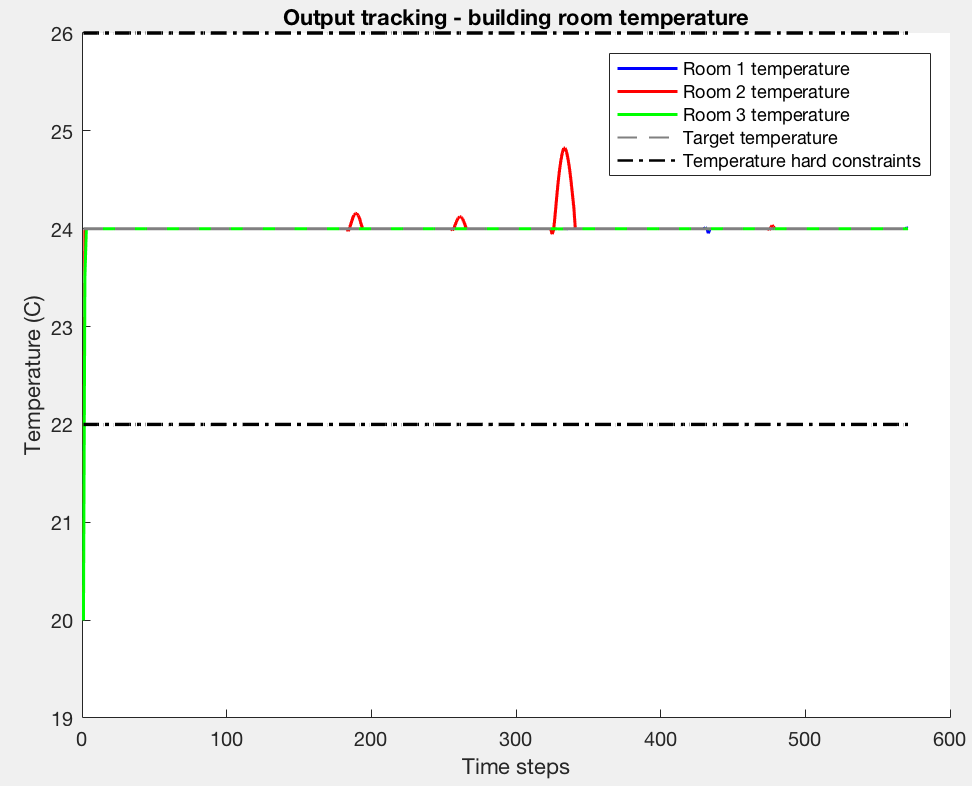
\includegraphics[width=\linewidth]{naivempc_N5_output}
				\caption{Output regulation, $N=5$}
				\label{fig::naivempc_N5_output}
			\end{minipage}
			\hfill
			\begin{minipage}{0.45\linewidth}
				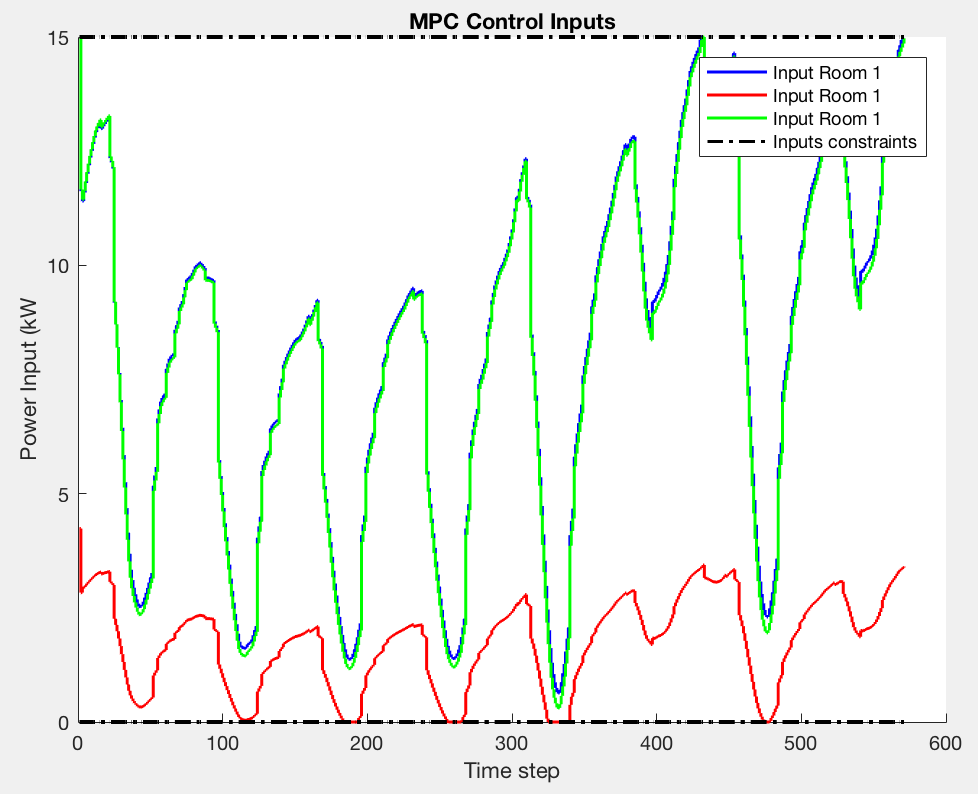
\includegraphics[width=\linewidth]{naivempc_N5_inputs}
				\caption{Inputs, $N=5$}
				\label{fig::naivempc_N5_inputs}
			\end{minipage}
		\end{figure}
		We can already note that all constraints are indeed verified. Because the disturbance is perfectly forecast (the disturbance applied is exactly the predicted one), the output tracking is done almost perfectly. We can indeed note that the temperature of the second room sometimes shows an overshoot. Because it is probably south-orientated, it is warmed up by the sun, which causes the room's temperature to rise, even if the input is zero. We can wonder what happens if we increase the prediction horizon so that the controller would be able to consider this raise in temperature. Figure (\ref{fig::naivempc_N20_output}) shows the rooms temperature for a controller of receeding horizon $N=20$. 
		\begin{figure}[ht!]
			\begin{center}
				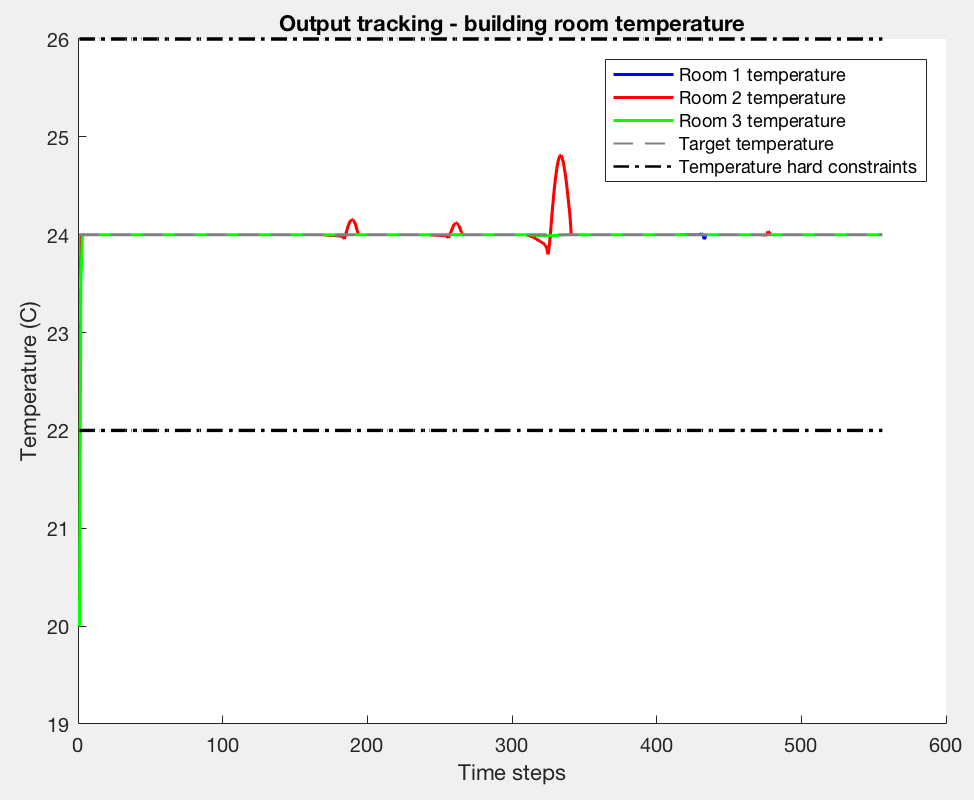
\includegraphics[width=0.5\linewidth]{naivempc_N20_output}
				\caption{Output regulation, $N=20$}
				\label{fig::naivempc_N20_output}
			\end{center}
		\end{figure}
		
		\paragraph{} Because the controller is now able to consider the temperature rise due to the orientation of the room and the sun exposition, it allows a small undershoot by setting the corresponding input to 0 well before this event. Therefore, a smaller undershoot is achieved when increasing the horizon, , since the room slightly cooled down before being being exposed to the sun. 

	}
   
   	\section{Economic MPC}
	{
		\paragraph{} We now wish to formulate our objective function as an economic function : given the electricity's price, we would like to minimize our bill. 
		\paragraph{} This implies switching to a linear cost function : 
		\begin{equation}
			J = C^T\left(\sum_{n=1}^N u_n\right)
		\end{equation}
		where $C=\begin{pmatrix} c & c & c\end{pmatrix}^T$ is a cost matrix, with $c=0.2$ \$/kWh. However, because this linear cost function might break some stability and recursive feasibility properties, a soft constraint formulation should be preferred. 
	}
	
	\section{Soft Constraints}
	{
	
		\begin{figure}[ht!]
			\begin{minipage}{0.45\linewidth}
				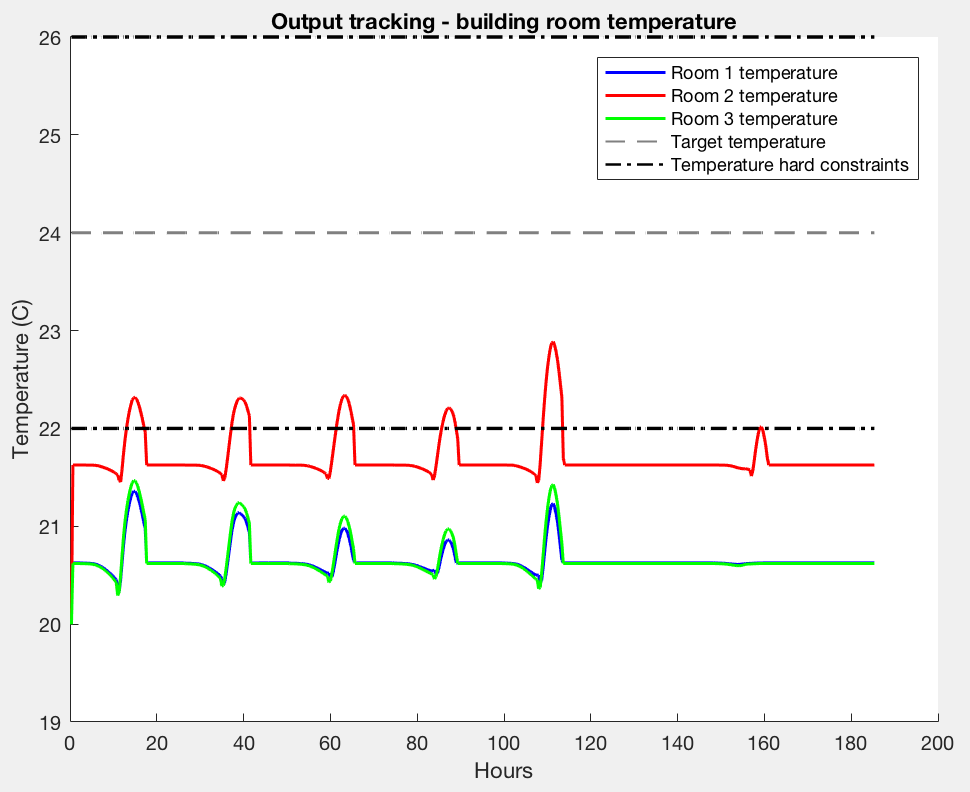
\includegraphics[width=\linewidth]{soft_constraints_01}
				\caption{Cost minimization with soft-constraints, $r_\eps=0.1$}
				\label{fig::soft_constraints_01}
			\end{minipage}
			\hfill
			\begin{minipage}{0.45\linewidth}
				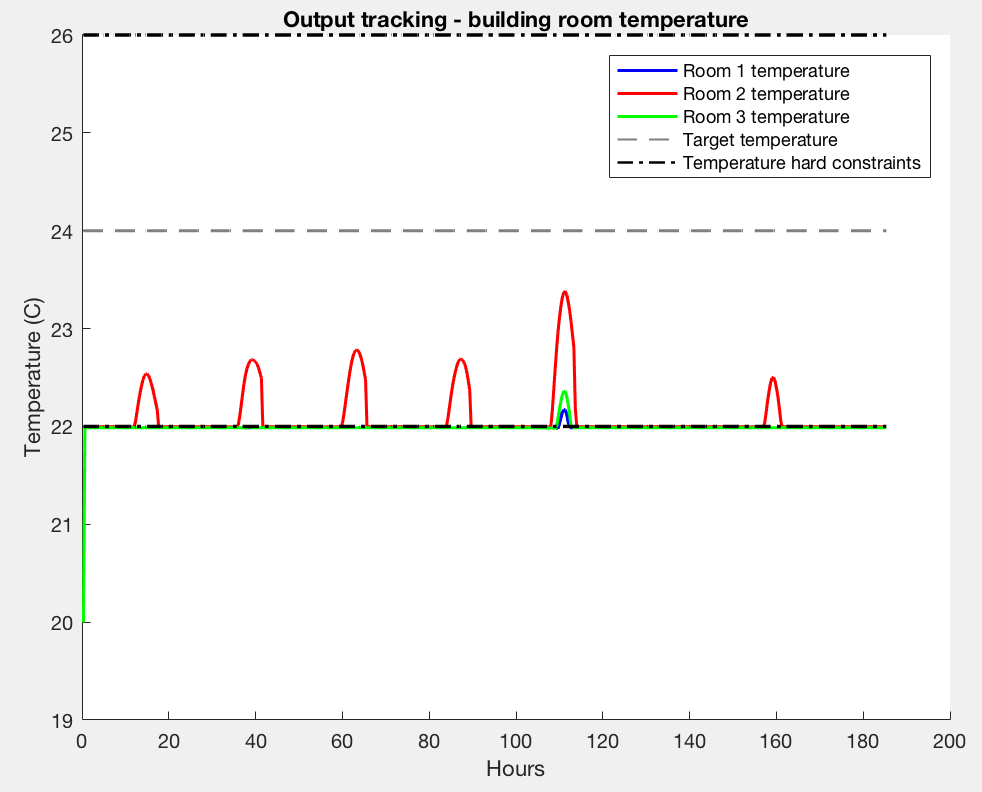
\includegraphics[width=\linewidth]{soft_constraints_10}
				\caption{Cost minimization with soft-constraints, $r_\eps=10$}
				\label{fig::soft_constraints_10}
			\end{minipage}
		\end{figure}
		
		\paragraph{} We hereinafter describe the soft constraints implementation of our controller and the obtained results. We decided to implement $L_2$ penalization for the slack variables, in order to limit constraints violation amplitude (a linear penalization would have penalized constraints violation duration instead). Indeed for comfort reasons, people in the rooms, would prefer to experience smaller deviation from the targeted temperature values for a long time than large deviation for small amounts of time. The actual optimization program we therefore solve writes : 
		\begin{mini}|s|[2]
  			{}{\sum_{n=1}^N\left[C^Tu_n +  r_\eps(\lVert \eps_n\rVert_2 +\lVert\hat{ \eps}_n\rVert_2)\right]}
  				 {\label{eq::svr}}{}
				 \addConstraint{y_n \geq 22 - \hat{\eps}_n}{\quad & &n\in\{1,\hdots,N\}}
				 \addConstraint{y_n \leq 26+\eps_n}{\quad & &n\in\{1,\hdots,N\}}
				 \addConstraint{u_n \leq 15}{\quad & &n\in\{1,\hdots,N\}}
				 \addConstraint{u_n \geq 0}{\quad & &n\in\{1,\hdots,N\}}
				 \addConstraint{\eps_n\geq 0}{\quad & &n\in\{1,\hdots,N\}}
				 \addConstraint{\hat{\eps}_n\geq 0}{\quad & &n\in\{1,\hdots,N\}}				 
		\end{mini}
		
		\paragraph{} Figures (\ref{fig::soft_constraints_01}) and (\ref{fig::soft_constraints_10}) display the results obtained with this controller, given an horizon size $N=20$, with two different penalization coefficient $r_\eps$. 
		\newline As one can expect, the retained solution's output stays near its lower bound, since this one corresponds to a lower cost. Also, by increasing the amplitude of the slack constraint amplitude, we reduce the size of the offset allowed by the tradeoff between constraints violation and cost minimization. 
		
	}
	
	\section{Variable Cost}
	{
	\begin{figure}[ht!]
			\begin{minipage}{0.45\linewidth}
				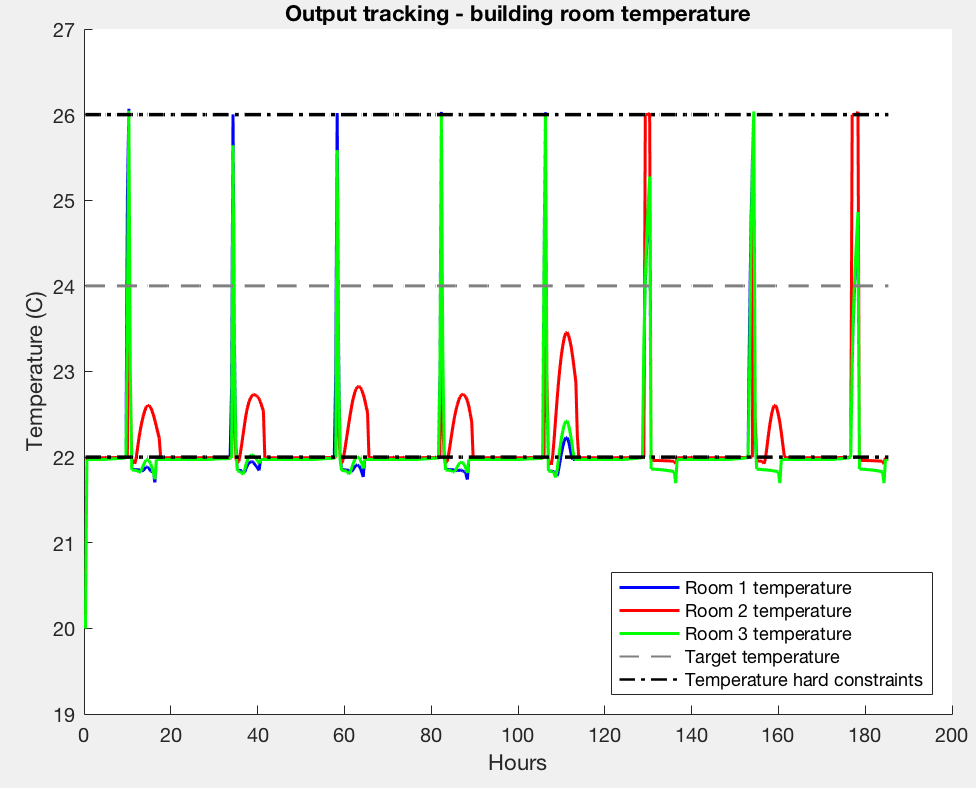
\includegraphics[width=\linewidth]{var_cost_output}
				\caption{Variable cost minimization, $r_\eps = 1$, $N = 20$}
				\label{fig::var_cost_output}
			\end{minipage}
			\hfill
			\begin{minipage}{0.45\linewidth}
				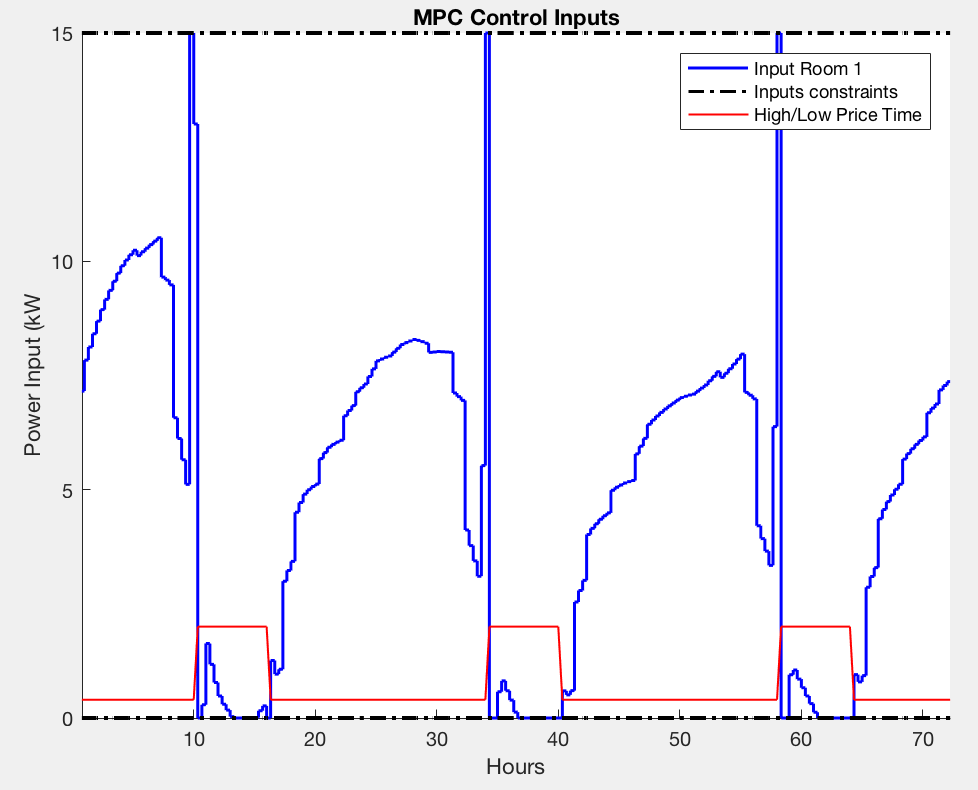
\includegraphics[width=\linewidth]{var_cost_inputs}
				\caption{Variable cost minimization, $r_\eps = 1$, $N = 20$}
				\label{fig::var_cost_inputs}
			\end{minipage}
		\end{figure}

		\paragraph{} We now wish to optimize a rather more realistic cost function, taking into account the variation of electricity prices. We consider the following model for the electricity prices : 
		\begin{equation}
			\begin{aligned}
				&c_k &= 0.2\$/kWh & &\quad \text{(between 12pm to 10am, and 4pm to 12pm)}\\
				&c_k &= 0.04\$/kWh & &\quad \text{(between 10:00Hrs to 16:00Hrs)}
			\end{aligned}
		\end{equation}
		This is achieved by specifying $c$ as a decision variable, provided at computation time. In the minimization problem, cost matrix is no longer constant so that it rewrites:
				\begin{mini}|s|[2]
  			{}{\sum_{n=1}^N\left[C_n^Tu_n +  r_\eps(\lVert \eps_n\rVert_2 +\lVert\hat{ \eps}_n\rVert_2)\right]}
  				 {\label{eq::svr}}{}
				 \addConstraint{y_n \geq 22 - \hat{\eps}_n}{\quad & &n\in\{1,\hdots,N\}}
				 \addConstraint{y_n \leq 26+\eps_n}{\quad & &n\in\{1,\hdots,N\}}
				 \addConstraint{u_n \leq 15}{\quad & &n\in\{1,\hdots,N\}}
				 \addConstraint{u_n \geq 0}{\quad & &n\in\{1,\hdots,N\}}
				 \addConstraint{\eps_n\geq 0}{\quad & &n\in\{1,\hdots,N\}}
				 \addConstraint{\hat{\eps}_n\geq 0}{\quad & &n\in\{1,\hdots,N\}}				 
				\end{mini}
		 
		where $C_n = [c_n, c_n, c_n]^T$.
		\paragraph{} In the following, we consider $r_\eps = 1$ as well as $N = 20$. Figure (\ref{fig::var_cost_output}) displays the evolution of temperature given this control strategy. We can namely see that, starting a few hours before the days rises, the temperature in the office increases before dropping. Figure (\ref{fig::var_cost_inputs}) gives a better insight at what is going on in the controller (for room 1). Indeed, we see that at the end of the night, the controller is provided with the prediction that the cost is soon to go up. To enable the constraints to be (softly) satisfied, without having to pay for expensive electricity in the morning, it peaks the input to warm up the different rooms. Therefore, during the day, it only has to buy a small amount of power to keep the temperature near its feasible region. 
	}
	
	\section{Night Setbacks}
	{
		\paragraph{} We will now implement time varying comfort constraints. The ideao is that outside of office hours, we would like to relax the output's constraints in order to safe money by avoiding unnecessary heating. Practically, we will consider the following constraints : 
		\begin{equation}
		\left\{
			\begin{aligned}
				&y^{max} = 30� & \quad& \text{between 12pm to 0am, and 6pm to 12pm} \\
				&y^{max} = 26� &\quad & \text{between 8am to 6pm} \\
				&y^{min} = 18� &\quad & \text{between 12pm to 0am, and 6pm to 12pm} \\
				&y^{min} = 22� & \quad& \text{between 8am to 6pm} \\
			\end{aligned}\right.
		\end{equation}
		
		
		Minimization problem therefore becomes:
		
						\begin{mini}|s|[2]
  			{}{\sum_{n=1}^N\left[C_n^Tu_n +  r_\eps(\lVert \eps_n\rVert_2 +\lVert\hat{ \eps}_n\rVert_2)\right]}
  				 {\label{eq::svr}}{}
				 \addConstraint{y_n \geq y^{min}_k - \hat{\eps}_n}{\quad & &n\in\{1,\hdots,N\}}
				 \addConstraint{y_n \leq y^{max}_k +\eps_n}{\quad & &n\in\{1,\hdots,N\}}
				 \addConstraint{u_n \leq 15}{\quad & &n\in\{1,\hdots,N\}}
				 \addConstraint{u_n \geq 0}{\quad & &n\in\{1,\hdots,N\}}
				 \addConstraint{\eps_n\geq 0}{\quad & &n\in\{1,\hdots,N\}}
				 \addConstraint{\hat{\eps}_n\geq 0}{\quad & &n\in\{1,\hdots,N\}}				 
				\end{mini}
		
		\begin{figure}[ht!]
			\begin{minipage}{0.45\linewidth}
				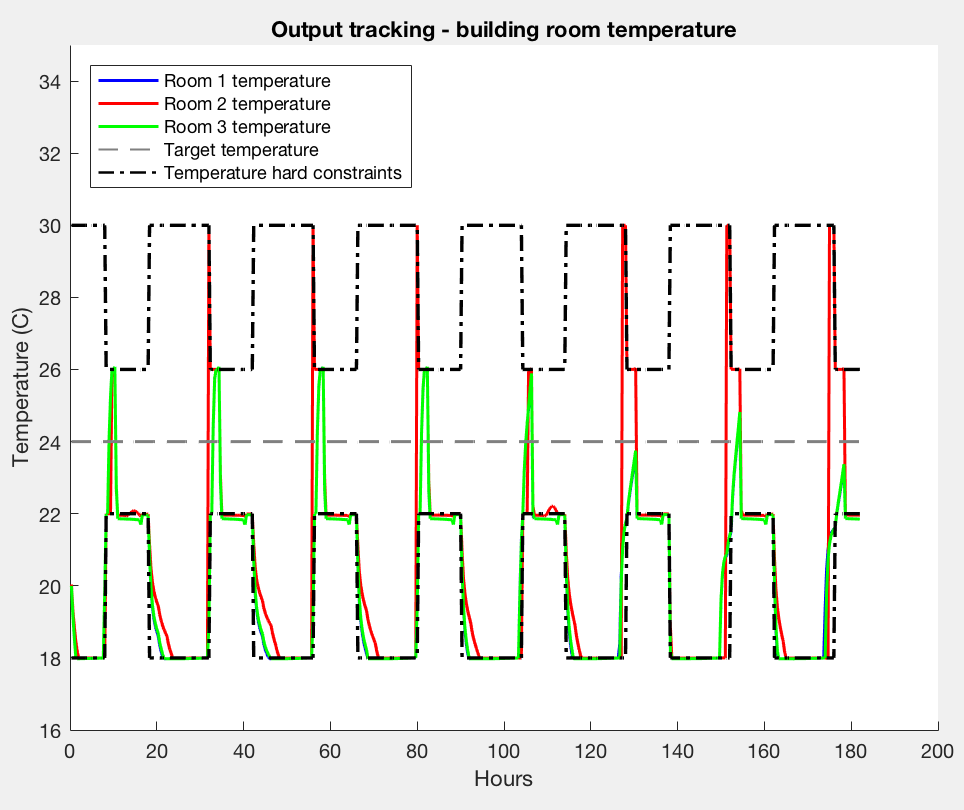
\includegraphics[width=\linewidth]{temp_setback}
				\caption{Variable cost minimization with night set-backs, $r_\eps = 1$, $N = 30$}
				\label{fig::temp_setback}
			\end{minipage}
			\hfill
			\begin{minipage}{0.45\linewidth}
				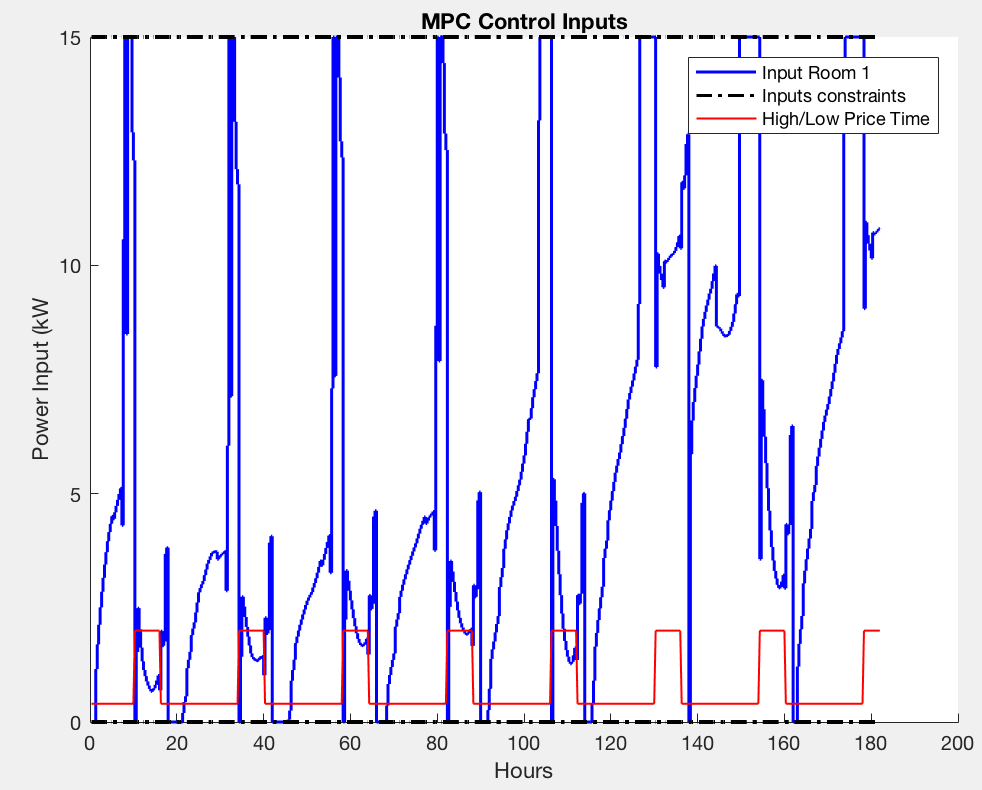
\includegraphics[width=\linewidth]{inputs_setback}
				\caption{Variable cost minimization with night-setbacks, $r_\eps = 1$, $N = 30$}
				\label{fig::inputs_setback}
			\end{minipage}
		\end{figure}


		\paragraph{} Figures (\ref{fig::temp_setback}) and (\ref{fig::inputs_setback})  respectively display the output (temperature) for the three different rooms (with the time varying constraints), as well as the input the the first room (alongside the cost zones). 
		\newline As one can notice, the temperature constraints are still met. More importantly, the controller let the temperature drop for most of the night (when no one is in office), before strongly heating  the building (taking advantage of the low cost of electricity by the end of the night). The temperature then drops when the employees begin in order to meet the actualized constraints. 
		\newline A slightly different behavior can be observed by the end of the available prediction time. Indeed, near hour 130, we can see that the controller imposes (unusual) stronger inputs in the morning. Indeed, because at that moment the solar gain are fairly weak and the outside temperature is rather cold, the controller needs to impose higher temperature in the morning before allowing it top drop to the lower-bound constraint. 
	}
	
	\section{Battery storage}
	{
		\paragraph{} In this section, we study the effect of having an electricity buffer (a battery) between the grid and the building. The charging power of the battery has lower and upper bound constraints. The idea is that we might be able to store cheap energy when it is cheap, and use that energy during the day, when buying it directly from the grid would be expensive. 
		
		\begin{figure}[ht!]
			\begin{minipage}{0.5\linewidth}
				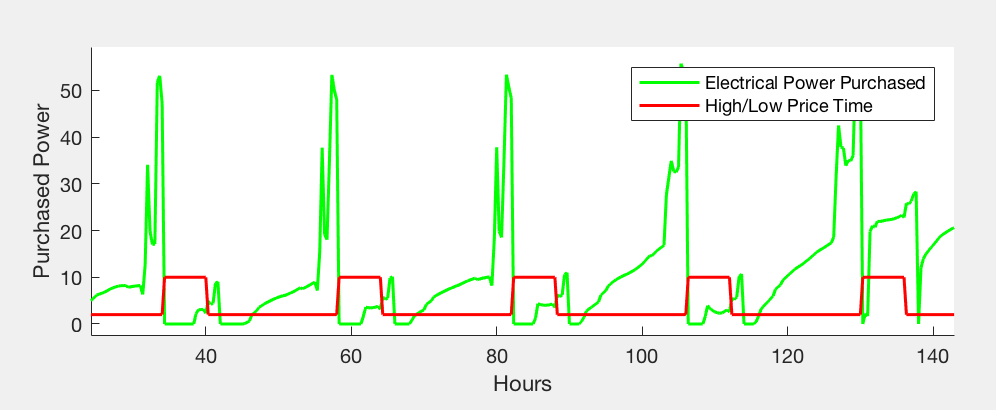
\includegraphics[width=\linewidth]{battery_purchase}
				\caption{Electrical power purchase ($N$=30)}
				\label{fig::battery_purchase}
			\end{minipage}
			\hfill
			\begin{minipage}{0.5\linewidth}
				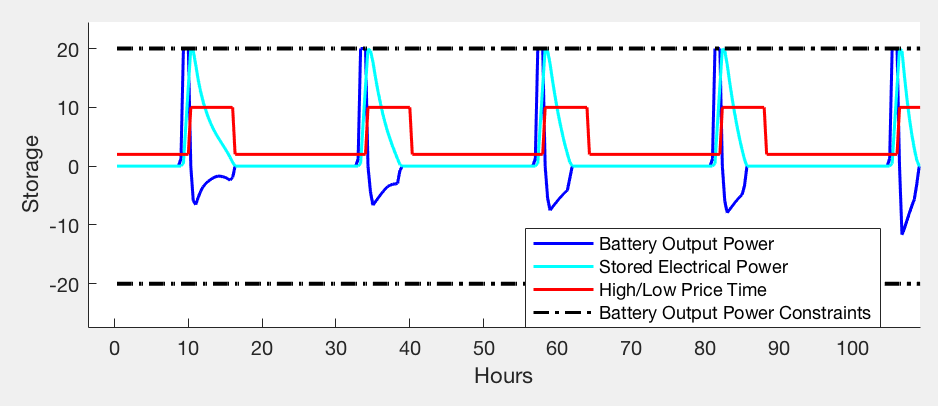
\includegraphics[width=\linewidth]{battery_charge}
				\caption{Battery's charging power and charge level ($N=30$)}
				\label{fig::battery_charge}
			\end{minipage}
		\end{figure}
		
		\begin{figure}[h!]
			\begin{center}
				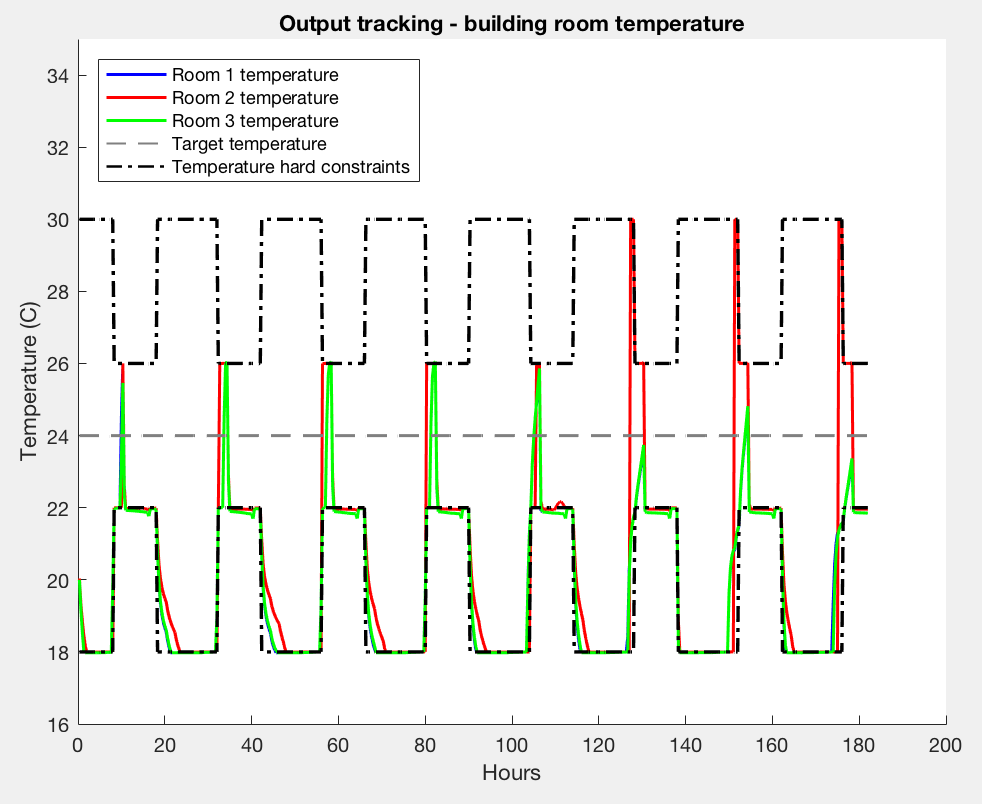
\includegraphics[width=0.5\linewidth]{battery_temp}
				\caption{Temperature evolution when using a battery ($N=20$)}
				\label{fig::temp_battery}
			\end{center}
		\end{figure}
		
		\paragraph{} Figures (\ref{fig::battery_purchase}) and (\ref{fig::battery_charge}) respectively display the power purchased from the grid and the charging power / capacity of the battery, along with the variation of the electrical power price. As expected, when internal gains, solar exposition, .. allow it, all most of the power is purchased when the price are low. Indeed, unlike when we did not consider this electricity buffer, some power was still needed during the day, when now almost none is bought at this period (this assertion becomes false when the battery storage is not enough to prevent temperature drops in the day - starting near hour 130). 
		\newline Also, one can notice that when electrical power is purchased, it is either use to directly warm the building or is stored in the battery. The battery discharges during the day, using the low price electricity that was bought the day before (figure (\ref{fig::battery_charge})). 
		
		\paragraph{} Figures (\ref{fig::temp_battery}) shows the system's output (temperature) variations. If we compare it with figures (\ref{fig::temp_setback}), we see that there is no more need for extreme (near saturation) heating by the end of the night. The controller simply needs to charge up the battery (it also warms the building to match the daytime temperature constraints) and discharge it during the day to keep the output inside its feasible region. The temperature in the building remains in the employees comfort zone, with much smoother dynamics. 
	}
\end{document}